14. а) Построим искомый треугольник по точкам пересечения данных прямых с осями координат: $(3;0),\ (0;2),\ (0;-2).$
$$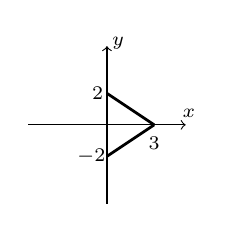
\begin{tikzpicture}[scale=0.2]
\tikzset {line01/.style={line width =0.5pt}}
\tikzset{line02/.style={line width =1pt}}
\tikzset{line03/.style={dashed,line width =0.5pt}}
%\filldraw [black] (0,0) circle (1pt);
\draw [->] (-5,0) -- (5,0);
\draw [->] (0,-5) -- (0,5);
\draw[line02] (3,0) -- (0,2);
\draw[line02] (3,0) -- (0,-2);
\draw[line02] (0,2) -- (0,-2);
\draw (5.2,0.7) node {\scriptsize $x$};
\draw (-0.6,2) node {\scriptsize $2$};
\draw (-1,-2) node {\scriptsize $-2$};
\draw (3,-1.2) node {\scriptsize $3$};
\draw (0.7,5.2) node {\scriptsize $y$};
\end{tikzpicture}$$
б) Все прямые вида $y=-x+b$ параллельны друг другу. Самая нижняя из них проходит через точку $(0;-2),$ поэтому $-2=0+b,\ b=-2$ --- наименьшее подходящее значение. Самая верхняя из них проходят через точку $(3;0),$ поэтому $0=-3+b,\ b=3$ --- наибольшее подходящее значение. Таким образом, $-2\leqslant b \leqslant 3.$\\
